\documentclass[11pt]{article}

\usepackage[bottom]{footmisc}

\usepackage{xcolor}
\usepackage{colortbl}

\usepackage{enumitem}

\usepackage{multicol}	

\usepackage{placeins}

\usepackage{hyperref}

\usepackage{caption}

\usepackage{amsmath, amsthm}

\usepackage{listings, lstautogobble}

\usepackage{tikz}
\usetikzlibrary{shapes,positioning,calc}

\title{COMP 6721: Artificial Intelligence,\\Project 2 Report}
\author{ Aria Adibi, 40139168}
\date{}

\definecolor{lightBlue}{RGB}{27, 168, 175}
\definecolor{darkishBlue}{RGB}{27, 71, 188}
\definecolor{darkishPurple}{RGB}{132, 14, 141}
\colorlet{lightgray}{gray!20}
\definecolor{codegreen}{rgb}{0,0.6,0}
\definecolor{codegray}{rgb}{0.5,0.5,0.5}
\definecolor{codepurple}{rgb}{0.58,0,0.82}

\hypersetup{
	colorlinks= true,
	linkcolor= darkishBlue,
%	anchorcolor= black,
	citecolor= black,
%	filecolor= cyan,
%	menucolor= red,
%	runcolor= cyan,
	urlcolor= lightBlue,
%	allcolors= black
}

\lstdefinestyle{mystyle}{
	keywordstyle=\color{darkishBlue},
	basicstyle=\small\ttfamily,
	commentstyle=\ttfamily\itshape\color{gray},
	stringstyle=\ttfamily\color{darkishPurple},
	%%%%%%%%%%%%%%%%%
	showspaces=false,                
	showstringspaces=false,
	showtabs=false,
	tabsize=3,
	%%%%%%%%%%%%%%%%%unknown
	%	frameround==ffff,
	%	breaklines=true,
	%	breakatwhitespace=false,
	%%%%%%%%%%%%%%%%%dose not wanted.
	%	frame=single,
	%	rulecolor=\color{black},
	%	backgroundcolor=\color{backcolour},
	%	numberstyle=\tiny\color{black},
	%	numbers=left,                    
	%	numbersep=5pt,
	%	captionpos=b,                    
	%	keepspaces=true,
	%%%%%%%%%%%%%%%%%
	autogobble=true
}

\lstdefinelanguage{ExSQL}{
	language= SQL,
	morekeywords=
	{TYPE, ENUM, ESCAPE, length, REFERENCES, REPLACE,
		FUNCTION, RETURNS, LANGUAGE, AFTER, FOR, EACH, ROW,
		PROCEDURE, BEGIN, RETURN, OFFSET, CEIL, RETURNING}
}

\lstset{style=mystyle}

%\renewcommand{\listfigurename}{}
%\renewcommand{\listtablename}{}
%\renewcommand\refname{}

%\setlength{\parindent}{4em}
\setlength{\parskip}{0.7em}
%\renewcommand{\baselinestretch}{2.0}

\newtheorem*{note}{Note}
\newtheorem*{definition}{Definition}

\begin{document}
	\maketitle
	
	\pagenumbering{roman}
	
	\begin{abstract}
		In this project the title of the posts of a popular site, \emph{HackersNews}, of the year 2019 is to be predicatively classifies into post types, given the data of the year 2018. The aim is to familiarize ourselves with the following:
		\begin{enumerate}
			\item
			How to parse texts and extract needed information in the context of Natural Language Processing
			\item
			To implement Naive Bayes algorithm, one of the easier (generative) classifiers in supervised learning algorithms.
			\item
			To investigate some of the easy modifications for performance improvements.
			
		\end{enumerate} 
	\end{abstract}
	
		%%%%%%%%%%%%%%%%%%%%%%%%%%%%%%%%%%%%%%%%%%%%%%%%
%	\thispagestyle{empty}
	\pagebreak %TODO
	\pagenumbering{gobble}
	
	\tableofcontents
%	\listoffigures
	\listoftables
	
	\newpage
	\pagenumbering{arabic}
	%%%%%%%%%%%%%%%%%%%%%%%%%%%%%%%%%%%%%%%%%%%%%%%%
	
	\section{ Introductions and technical details }
		\subsection{ Introduction }
			Following information of posts in a popular site, HackersNews, for the years 2018 and 2019 is given.
			
			\begin{centering}
				\begin{tabular}{ | c | c | c | c | c | c | c | c |}
					\hline
					Object ID & Title & Post Type & Author & Created At & URL & ... \\
					\hline
					... & Points & Number of Comments \\
					\cline{1-3}
				\end{tabular}
			\end{centering}
			
			The chosen supervised model is Naive Bayes, which has to predict the Post Type given the Title. The training data is the ones created at 2018 and the test data is the 2019 ones.
			
			My code first parse the given \texttt{.csv} file and extract the useful information, with the help of \texttt{NLTK} package.
			
			Then the Naive Bayes algorithm is implemented. At the end some tweaks are investigated to study their effects on performance and accuracy.
			
		\subsection{Technical details}
			In the provided \texttt{.zip} file you will find the following files:
			\begin{itemize}
				\item {\ttfamily README.txt}\\
					This \texttt{.txt} file provides the instructions needed to run the program.
				\item {\ttfamily main\_v1.py}\\
					The main (runnable) python module which is to be executed.
				\item {\ttfamily Technical Report}\\
					This file, which reports and give analysis of the project.
				\item {\ttfamily Expectation of Originality}\\
					A signed form for the purpose of originality of the work.
			\end{itemize}
	%%%%%%%%%%%%%%%%%%%%%%%%%%%%%%%%%%%%%%%%%%%%%%%%	
	\section{Explanation of the parsing and extraction part}
		\subsection{Observation}
			By manually observing the data, one can see that the data has no missing values, therefore no \texttt{imputation} is needed.
			Also the data seems balanced with no mistake.
		
		\subsection{The methodology}
		After reading the \texttt{.csv} file and separating the columns, the additional information is removed and data is parted in two sets: Training and Testing.
		With the help of the \texttt{NLTK} package then the data in Title column was \texttt{tokenized}. One could tokenize proper names such as ``Computer Science''
		as one item with the tags associated in the when NLTK parses the text. At the same time ``stop words'' are removed and the frequency of words and their post-type-conditional
		frequency is accumulated. At the end a smoothed probability (for resolving zero probability issue) is associated. 
		
		The smoothing function used is \emph{Additive Smoothing}, also called \emph{Laplace smoothing}, with its ``psedocount'' set to $0.5$.
		
	\section{Results and their analyzation }
		\subsection{Naive Bayes Model}
			\textbf{Bayes Theorem:}
			\textit{Let $\{B_1,\ B_2,\ \ldots, B_n\}$ be a partition of the sample space $S$ of the experiment. If for $i=\ 1,\ 2,\ \ldots,\ n,\ \ P(B_i) > 0$, then for
			any event $A$ of $S$ with $P(A) > 0$,
				$$ P(B_k | A) = \frac{P(A | B_k) P(B_k)}{ \Sigma_{i=1}^{n}  P(A | B_i) P(B_i)} $$
			}
				
			Assuming the ``Naive'' assumption that the features (here words of a given title) of the model are independent, and the fact that our classes (here Post Types) partition
			our sample space one can use Bayes theorem to calculate the probability of a title belonging to each class. The higher one is the prediction of the algorithm.
			
		\subsection{Results}
			The files containing the results are provided as requested in the project description, with a diagram shown after running the algorithm and acuuracy reported in terminal.
			
					\begin{figure}[h!]
						\centering
						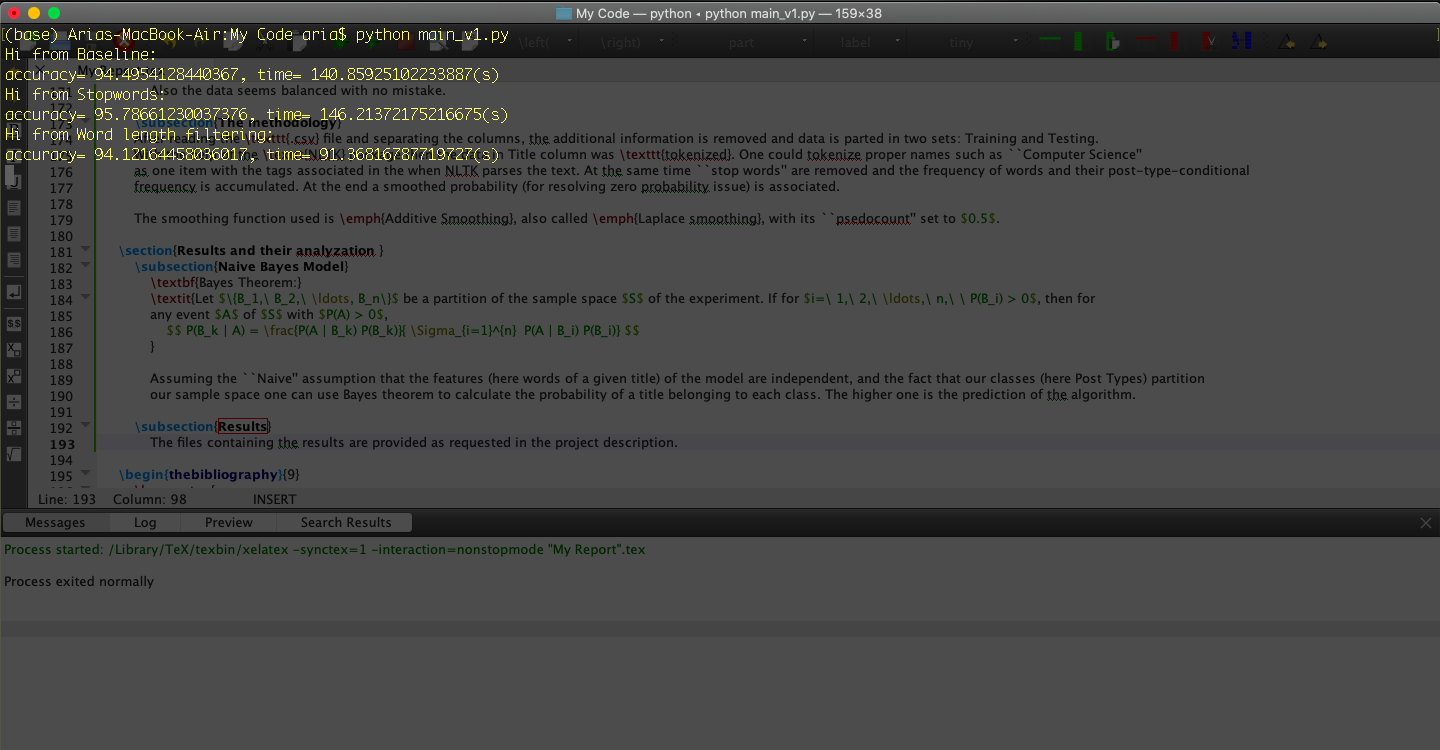
\includegraphics[width= 0.50\textwidth]{./Images/1.png}
						\caption{Example of the terminal report}
					\end{figure}

					\begin{figure}[h!]
						\centering
						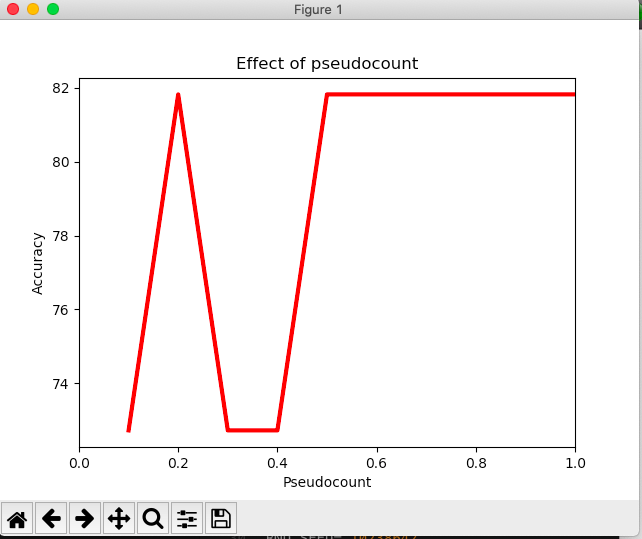
\includegraphics[width= 0.50\textwidth]{./Images/2.png}
						\caption{Example of the shown diagram}
					\end{figure}		
	\begin{thebibliography}{9}
		\hypersetup{
			urlcolor= black
		}
			\bibitem{}
	\end{thebibliography}

\end{document}

%		\ref{fig:DesignPhasesDB}

%		\cite[p. 61]{FundDB}.

%		\begin{figure}[h!]
%			\centering
%			\includegraphics[width= 0.85\textwidth]{./Images/mainPhasesOfTheDesign.png}
%			\caption[name in caption] 
%				{the caption}
%			\label{fig:DesignPhasesDB}
%		\end{figure}

%		\footnote{conceptual modeling}


%		\begin{itemize}
%			\item[-]
%			{\bfseries
%				some item
%			}\\
%		\end{itemize}

%\begin{enumerate}
%	\item
%	A
%\end{enumerate}

%\newtheorem*{remark}{Remark}
%\begin{remark}
%	remark
%\end{remark}

%		\newtheorem*{definition}{Definition}
%		\begin{definition}
%			\setlength{\leftskip}{0.9cm}
%			A relation schema $R$ is in 
%			{\bfseries first normal form (1NF)} if it has no multivalued
%			or nested relations; in another words all of it's attributes
%			are atomic.
%		\end{definition}
%		\begin{definition}
%			\setlength{\leftskip}{0.9cm}
%			A relation schema $R$ is in 
%			{\bfseries second normal form (2NF)} if every nonprime
%			attribute $A$ in $R$ is not partially dependent on any key
%			of $R$.
%		\end{definition}
%		\begin{definition}
%			\setlength{\leftskip}{0.9cm}
%			A relation schema $R$ is in
%			{\bfseries third normal form (3NF)} if, whenever a nontrivial
%			functional dependency $X \rightarrow A$ holds in $R$, either
%			(a) $X$ is a superkey of $R$, or (b) $A$ is a prime attribute
%			of $R$.
%		\end{definition}
%		\begin{definition}
%			\setlength{\leftskip}{0.9cm}
%			A relation schema $R$ is in {\bfseries BCNF} if whenever 
%			a nontrivial functional dependency $X \rightarrow A$ holds
%			in $R$, then $X$ is a superkey of $R$.
%		\end{definition}

%\section{Section}
%\subsection{SubSection}
%\subsubsection{SubSubSection} \label{dataRequirmentsProj1}
%\cite{typeTotorialsPoint}

%{\bfseries \texttt{Coupon} }\\
%\begin{tabular}{|l|l|}
%	\hline
%	
%	\texttt{category:: couponCategories*} & \texttt{description:: text}\\
%	\hline
%	
%	\texttt{lineaments:: text} & \texttt{companyName:: nameDomain*}\\
%	\hline
%	
%	\texttt{companyAddress:: text} & \texttt{conditions:: text}\\
%	\hline
%	
%	\multicolumn{2}{|l|}{ \texttt{nameAndAShortDescription:: character varying(150)} }\\
%	\hline
%	
%	\texttt{numOfCoupons:: integer} & \texttt{numOfSoldCoupons:: integer}\\
%	\hline
%	
%	\texttt{originalPrice:: money} & \texttt{percentageOff:: integer}\\
%	\hline
%	
%	\texttt{expirationDate:: date} & \texttt{id:: serial}\\
%	\hline
%\end{tabular}
%%		\captionof{}
%%			{}
%\label{table:typeCoupon}

%\begin{center}
%	\setlength\arrayrulewidth{0.8pt}
%	\begin{tabular}{|l|c|}
%		\hline
%		\rowcolor{lightgray}
%		\multicolumn{1}{|c|}{\bfseries Limit} & 
%		{\bfseries Value}\\
%		\hline
%		Maximum Database & unlimited\\
%		\hline
%		Maximum Table Size & 32 terabyte\\
%		\hline
%		Maximum Row Size & 1.6 terabyte\\
%		\hline
%		Maximum Rows per Table & unlimited\\
%		\hline
%		Maximum Columns per Table & 1600-2500 depending on column types\\
%		\hline
%		Maximum Indexes per Table & unlimited\\
%		\hline
%	\end{tabular}
%	\captionof{table}[]
%	{}
%	\label{table:limitationsOfPostgrSQL}
%\end{center}

%\begin{lstlisting}[language= ExSQL]
%CREATE TYPE "couponCategories" AS ENUM
%('RESTAURANT_COFFEESHOP',
%'ART_THEATER',
%'ENTERTAINMENT_SPORT',
%'EDUCATIONAL',
%'HEALTH_MED',
%'COSMETIC',
%'TRAVEL',
%'GOODS');
%\end{lstlisting}

%\begin{figure}[h!]
%	\centering
%	\begin{tikzpicture}[relation/.style={rectangle split, rectangle split parts=#1, rectangle split part align=base, draw, anchor=center, align=center, text height=2mm, text centered}]
%	\end{tikzpicture}
%	\caption[NAME IN TABLE]
%	{}
%	\label{fig:FDRProj1}
%\end{figure}